%%%%%%%%%%%%%%%%%%%%%%%%%%%%%%%%%%%%%%%%%
% Cleese Assignment (For Students)
% LaTeX Template
% Version 2.0 (27/5/2018)
%
% This template originates from:
% http://www.LaTeXTemplates.com
%
% Author:
% Vel (vel@LaTeXTemplates.com)
%
% License:
% CC BY-NC-SA 3.0 (http://creativecommons.org/licenses/by-nc-sa/3.0/)
% 
%%%%%%%%%%%%%%%%%%%%%%%%%%%%%%%%%%%%%%%%%

%----------------------------------------------------------------------------------------
%	PACKAGES AND OTHER DOCUMENT CONFIGURATIONS
%----------------------------------------------------------------------------------------

\documentclass[11pt]{article}

%%%%%%%%%%%%%%%%%%%%%%%%%%%%%%%%%%%%%%%%%
% Cleese Assignment
% Structure Specification File
% Version 1.0 (27/5/2018)
%
% This template originates from:
% http://www.LaTeXTemplates.com
%
% Author:
% Vel (vel@LaTeXTemplates.com)
%
% License:
% CC BY-NC-SA 3.0 (http://creativecommons.org/licenses/by-nc-sa/3.0/)
% 
%%%%%%%%%%%%%%%%%%%%%%%%%%%%%%%%%%%%%%%%%

%----------------------------------------------------------------------------------------
%	PACKAGES AND OTHER DOCUMENT CONFIGURATIONS
%----------------------------------------------------------------------------------------

\usepackage{lastpage} % Required to determine the last page number for the footer

\usepackage{graphicx} % Required to insert images

\setlength\parindent{0pt} % Removes all indentation from paragraphs

\usepackage[most]{tcolorbox} % Required for boxes that split across pages

\usepackage{booktabs} % Required for better horizontal rules in tables

\usepackage{listings} % Required for insertion of code

\usepackage{etoolbox} % Required for if statements


%----------------------------------------------------------------------------------------
%	MARGINS
%----------------------------------------------------------------------------------------

\usepackage{geometry} % Required for adjusting page dimensions and margins

\geometry{
	paper=a4paper, % Change to letterpaper for US letter
	top=3cm, % Top margin
	bottom=3cm, % Bottom margin
	left=2.5cm, % Left margin
	right=2.5cm, % Right margin
	headheight=14pt, % Header height
	footskip=1.4cm, % Space from the bottom margin to the baseline of the footer
	headsep=1.2cm, % Space from the top margin to the baseline of the header
	%showframe, % Uncomment to show how the type block is set on the page
}

%----------------------------------------------------------------------------------------
%	FONT
%----------------------------------------------------------------------------------------

\usepackage[utf8]{inputenc} % Required for inputting international characters
\usepackage[T1]{fontenc} % Output font encoding for international characters

\usepackage[sfdefault,light]{roboto} % Use the Roboto font

%----------------------------------------------------------------------------------------
%	HEADERS AND FOOTERS
%----------------------------------------------------------------------------------------

\usepackage{fancyhdr} % Required for customising headers and footers

\pagestyle{fancy} % Enable custom headers and footers

\lhead{\small\assignmentClass\ifdef{\assignmentClassInstructor}{\ (\assignmentClassInstructor):}{}\ \assignmentTitle} % Left header; output the instructor in brackets if one was set
\chead{} % Centre header
\rhead{\small\ifdef{\assignmentAuthorName}{\assignmentAuthorName}{\ifdef{\assignmentDueDate}{Due\ \assignmentDueDate}{}}} % Right header; output the author name if one was set, otherwise the due date if that was set

\lfoot{} % Left footer
\cfoot{\small Page\ \thepage\ of\ \pageref{LastPage}} % Centre footer
\rfoot{} % Right footer

\renewcommand\headrulewidth{0.5pt} % Thickness of the header rule

%----------------------------------------------------------------------------------------
%	MODIFY SECTION STYLES
%----------------------------------------------------------------------------------------

\usepackage{titlesec} % Required for modifying sections

%------------------------------------------------
% Section

\titleformat
{\section} % Section type being modified
[block] % Shape type, can be: hang, block, display, runin, leftmargin, rightmargin, drop, wrap, frame
{\Large\bfseries} % Format of the whole section
{\assignmentQuestionName~\thesection} % Format of the section label
{6pt} % Space between the title and label
{} % Code before the label

\titlespacing{\section}{0pt}{0.5\baselineskip}{0.5\baselineskip} % Spacing around section titles, the order is: left, before and after

%------------------------------------------------
% Subsection

\titleformat
{\subsection} % Section type being modified
[block] % Shape type, can be: hang, block, display, runin, leftmargin, rightmargin, drop, wrap, frame
{\itshape} % Format of the whole section
{(\alph{subsection})} % Format of the section label
{4pt} % Space between the title and label
{} % Code before the label

\titlespacing{\subsection}{0pt}{0.5\baselineskip}{0.5\baselineskip} % Spacing around section titles, the order is: left, before and after

\renewcommand\thesubsection{(\alph{subsection})}

%----------------------------------------------------------------------------------------
%	CUSTOM QUESTION COMMANDS/ENVIRONMENTS
%----------------------------------------------------------------------------------------

% Environment to be used for each question in the assignment
\newenvironment{question}{
	\vspace{0.5\baselineskip} % Whitespace before the question
	\section{} % Blank section title (e.g. just Question 2)
	\lfoot{\small\itshape\assignmentQuestionName~\thesection~continued on next page\ldots} % Set the left footer to state the question continues on the next page, this is reset to nothing if it doesn't (below)
}{
	\lfoot{} % Reset the left footer to nothing if the current question does not continue on the next page
}

%------------------------------------------------

% Environment for subquestions, takes 1 argument - the name of the section
\newenvironment{subquestion}[1]{
	\subsection{#1}
}{
}

%------------------------------------------------

% Command to print a question sentence
\newcommand{\questiontext}[1]{
	\textbf{#1}
	\vspace{0.5\baselineskip} % Whitespace afterwards
}

%------------------------------------------------

% Command to print a box that breaks across pages with the question answer
\newcommand{\answer}[1]{
	\begin{tcolorbox}[breakable, enhanced]
		#1
	\end{tcolorbox}
}

%------------------------------------------------

% Command to print a box that breaks across pages with the space for a student to answer
\newcommand{\answerbox}[1]{
	\begin{tcolorbox}[breakable, enhanced]
		\vphantom{L}\vspace{\numexpr #1-1\relax\baselineskip} % \vphantom{L} to provide a typesetting strut with a height for the line, \numexpr to subtract user input by 1 to make it 0-based as this command is
	\end{tcolorbox}
}

%------------------------------------------------

% Command to print an assignment section title to split an assignment into major parts
\newcommand{\assignmentSection}[1]{
	{
		\centering % Centre the section title
		\vspace{2\baselineskip} % Whitespace before the entire section title
		
		\rule{0.8\textwidth}{0.5pt} % Horizontal rule
		
		\vspace{0.75\baselineskip} % Whitespace before the section title
		{\LARGE \MakeUppercase{#1}} % Section title, forced to be uppercase
		
		\rule{0.8\textwidth}{0.5pt} % Horizontal rule
		
		\vspace{\baselineskip} % Whitespace after the entire section title
	}
}

%----------------------------------------------------------------------------------------
%	TITLE PAGE
%----------------------------------------------------------------------------------------

\author{\textbf{\assignmentAuthorName}} % Set the default title page author field
\date{} % Don't use the default title page date field

\title{
	\thispagestyle{empty} % Suppress headers and footers
	\vspace{0.2\textheight} % Whitespace before the title
	\textbf{\assignmentClass:\ \assignmentTitle}\\[-4pt]
	\ifdef{\assignmentDueDate}{{\small Due\ on\ \assignmentDueDate}\\}{} % If a due date is supplied, output it
	\ifdef{\assignmentClassInstructor}{{\large \textit{\assignmentClassInstructor}}}{} % If an instructor is supplied, output it
	\vspace{0.32\textheight} % Whitespace before the author name
}
 % Include the file specifying the document structure and custom commands
\usepackage{ctex}
\usepackage{tabularx}
\usepackage{booktabs}
\usepackage{graphicx}
\usepackage{caption}
\usepackage{subcaption}
\usepackage{float}
%----------------------------------------------------------------------------------------
%	ASSIGNMENT INFORMATION
%----------------------------------------------------------------------------------------

% Required
\newcommand{\assignmentQuestionName}{Problem} % The word to be used as a prefix to question numbers; example alternatives: Problem, Exercise
\newcommand{\assignmentClass}{ZJU Computational Physics} % Course/class
\newcommand{\assignmentTitle}{Homework\ \#2} % Assignment title or name
\newcommand{\assignmentAuthorName}{NAKO} % Student name

% Optional (comment lines to remove)
%\newcommand{\assignmentClassInstructor}{} % Intructor name/time/description
\newcommand{\assignmentDueDate}{Monday,\ December\ 2,\ 2024\\
Github: https://github.com/NAKONAKO4/ZJU-computational-physics-NAKO} % Due date
\usepackage{listings, xcolor}
\lstdefinestyle{lfonts}{
  basicstyle   = \footnotesize\ttfamily,
  stringstyle  = \color{purple},
  keywordstyle = \color{blue!60!black}\bfseries,
  commentstyle = \color{olive}\scshape,
}
\lstdefinestyle{lnumbers}{
  numbers     = left,
  numberstyle = \tiny,
  numbersep   = 1em,
  firstnumber = 1,
  stepnumber  = 1,
}
\lstdefinestyle{llayout}{
  breaklines       = true,
  tabsize          = 2,
  columns          = flexible,
}
\lstdefinestyle{lgeometry}{
  xleftmargin      = 20pt,
  xrightmargin     = 0pt,
  frame            = tb,
  framesep         = \fboxsep,
  framexleftmargin = 20pt,
}
\lstdefinestyle{lgeneral}{
  style = lfonts,
  style = lnumbers,
  style = llayout,
  style = lgeometry,
}
\lstdefinestyle{python}{
  language = {Python},
  style    = lgeneral,
}
%----------------------------------------------------------------------------------------

\begin{document}

%----------------------------------------------------------------------------------------
%	TITLE PAGE
%----------------------------------------------------------------------------------------

\maketitle % Print the title page

\thispagestyle{empty} % Suppress headers and footers on the title page

\newpage

%----------------------------------------------------------------------------------------
%	QUESTION 1
%----------------------------------------------------------------------------------------

\begin{question}

\questiontext{Derivatives}
\answer{将forward formula, central difference formula, Richardson extrapolation结果绘制在图中进行对比。}
\lstinputlisting[style = python]{1/a.py}
\answer{运行结果为}
\begin{center}
	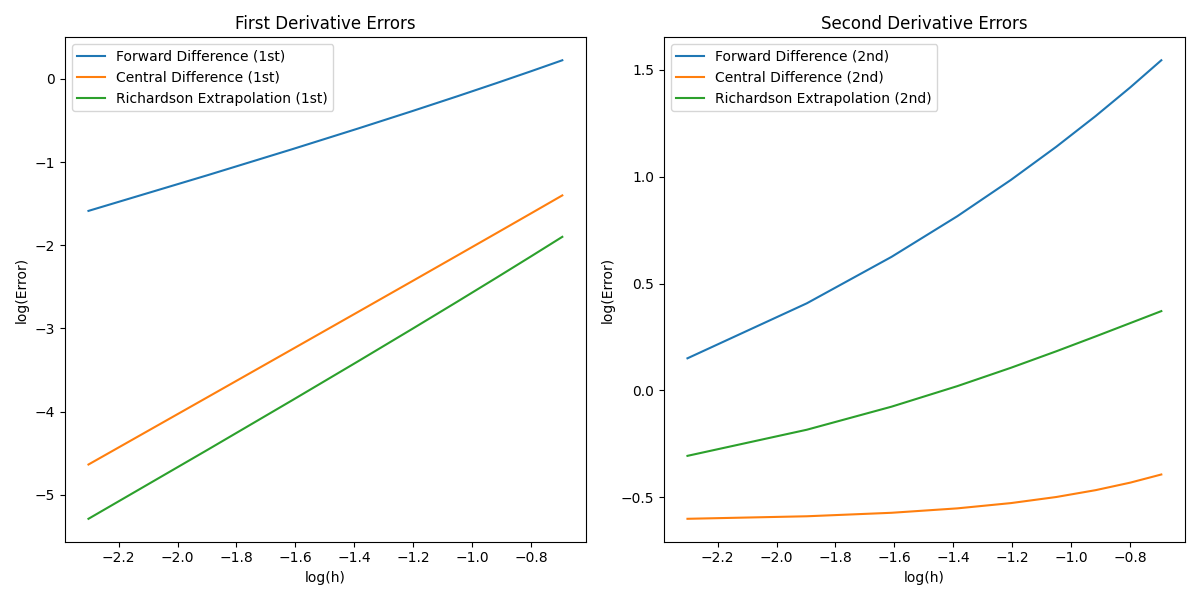
\includegraphics[width=\columnwidth]{1/a1.png}
\end{center}
\answer{b. 参见/1/b.py,图像中可见仍然存在一定的与实际值的误差。
		
		运行结果为
		}
\begin{center}
	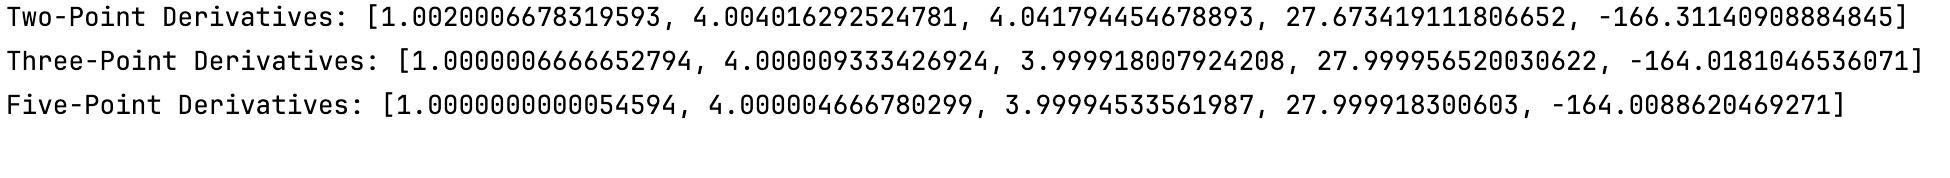
\includegraphics[width=\columnwidth]{1/b1.png}
\end{center}
\lstinputlisting[style = python]{1/b.py}
\end{question}

%----------------------------------------------------------------------------------------
%	QUESTION 2
%----------------------------------------------------------------------------------------

\begin{question}

\questiontext{Integration}
\lstinputlisting[style = python]{2/a.py}
\answer{运行结果为:

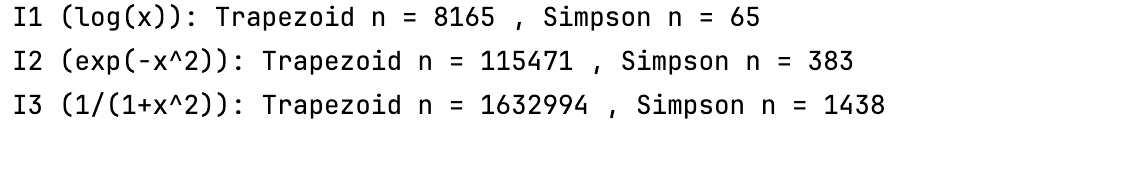
\includegraphics[width=\columnwidth]{2/a1.png}

		整理如下}

\begin{table}[h]
	\centering
	\begin{tabular}{l l l}
		\toprule
		&Trapezoid n& Simpson n\\
		\midrule
		$I_1 (log(x))$&8165&65\\
		$I_2 (exp(-x^2))$&115471&383\\
		$I_3 (1/(1+x^2))$&1632994&1438\\
		\bottomrule
	\end{tabular}
\end{table}
%--------------------------------------------
%--------------------------------------------

\end{question}
%--------------------------------------------
% question 3
%--------------------------------------------
\begin{question}
\questiontext{Hilbert Matrix}
\answer{通过python numpy库的linalg.eigvals()函数可以直接将矩阵对角化并计算出矩阵的特征值。本题目使用了numpy库的linalg.eigvals()函数来对角化矩阵并计算特征值。}
\lstinputlisting[style = python]{3/a.py}
\begin{center}
	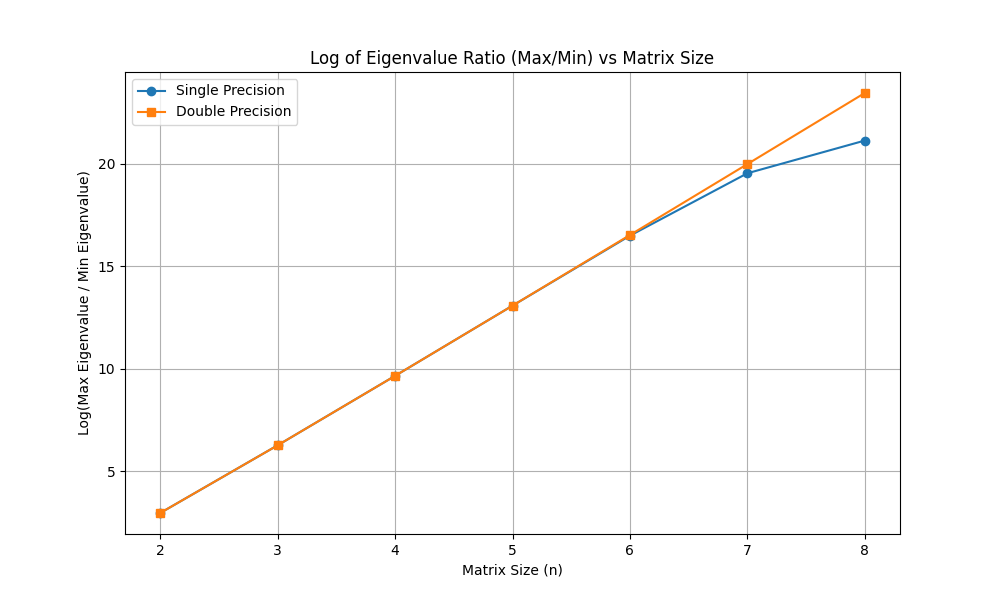
\includegraphics[width=\columnwidth]{3/a1.png}
\end{center}
\end{question}

%--------------------------------------------
% question 4
%--------------------------------------------
\begin{question}
\questiontext{Coupled Oscillators}
\answer{a. 设置耦合系数为1,每个振子的质量为1,在T=10的模拟时长进行计算。首先通过欧拉方法来求解数值解,并与通过模态展开得到的解析解结果的$u_j(t)$进行对比。可以得到结果为}
\begin{center}
	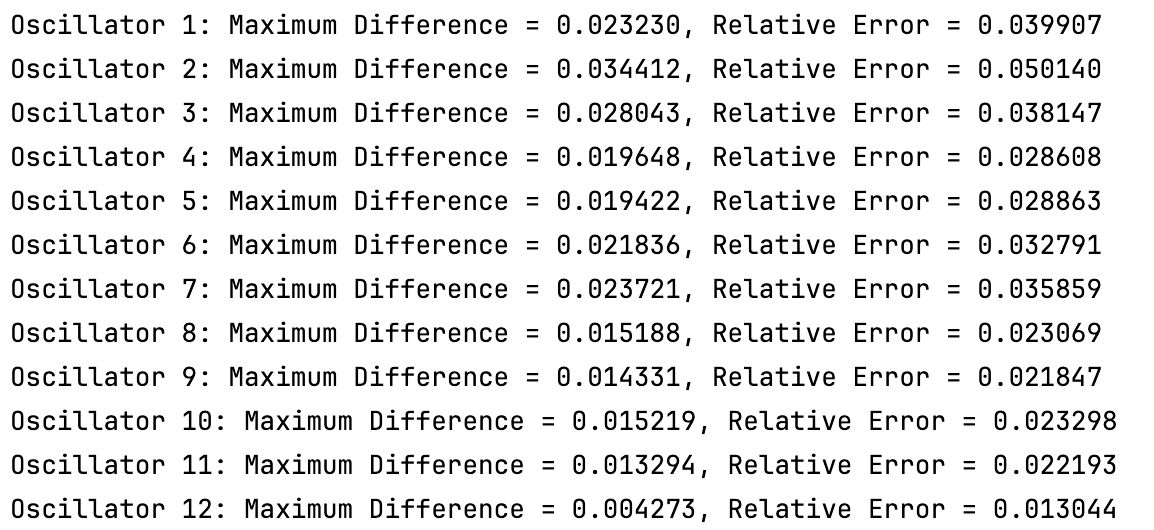
\includegraphics[width=\columnwidth]{4/a1_1.png}
\end{center}
\answer{可以看到,欧拉方法得到的差值结果较大,相对误差较大。\par
		于是我又尝试了用Runge-Kutta 4th方法去进行上述计算,得到结果如下}
		\begin{center}
			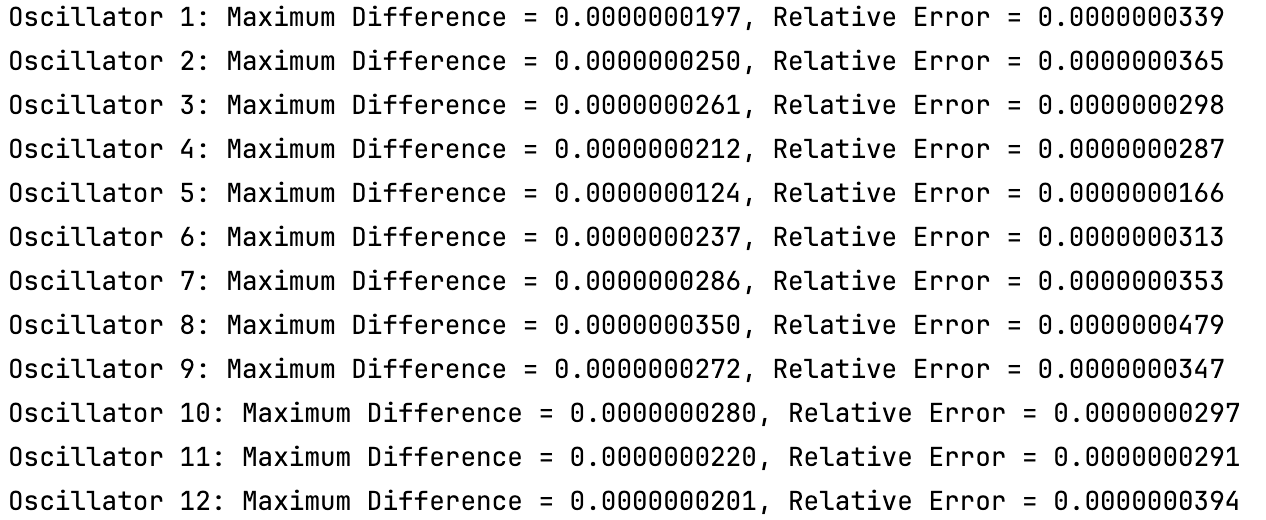
\includegraphics[width=\columnwidth]{4/a2_1.png}
		\end{center}
\answer{可以看到Runge-Kutta 4th方法得到的精度明显高于欧拉方法。}
\answer{欧拉方法}
\lstinputlisting[style = python]{4/a1.py}
\answer{Runge-Kutta 4th方法}
\lstinputlisting[style = python]{4/a1_1.py}
\answer{b. 采用欧拉方法计算,得到结果如下}
\begin{center}
	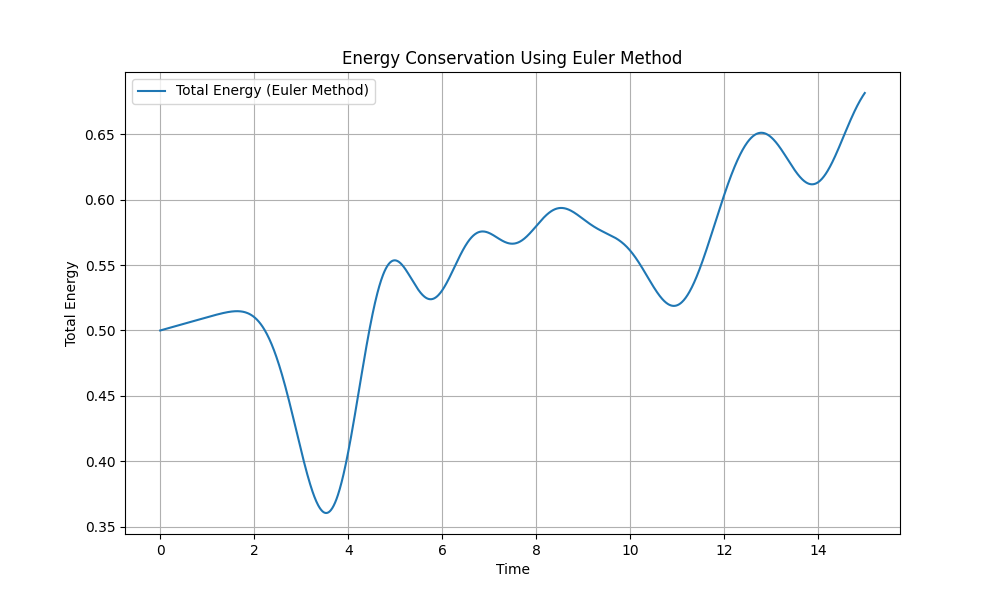
\includegraphics[width=\columnwidth]{4/b2.png}
\end{center}
\answer{但事实上与解析解能量进行对比可以看到,欧拉方法与解析解能量并不吻合。}
\begin{center}
	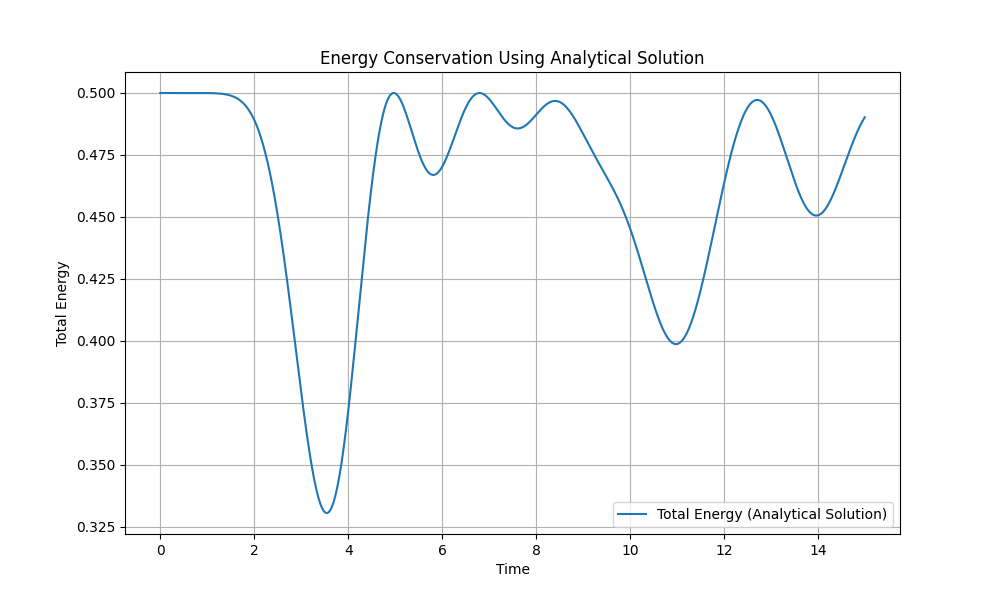
\includegraphics[width=\columnwidth]{4/b1.png}
\end{center}
\answer{同时也可以看到,在更长的时间上进行计算,解析解的能量守恒并不是很好,在初始能量0.5下面波动,但是均值还是在0.475附近,存在一些比较大的波动到达0.375附近。}
\begin{center}
	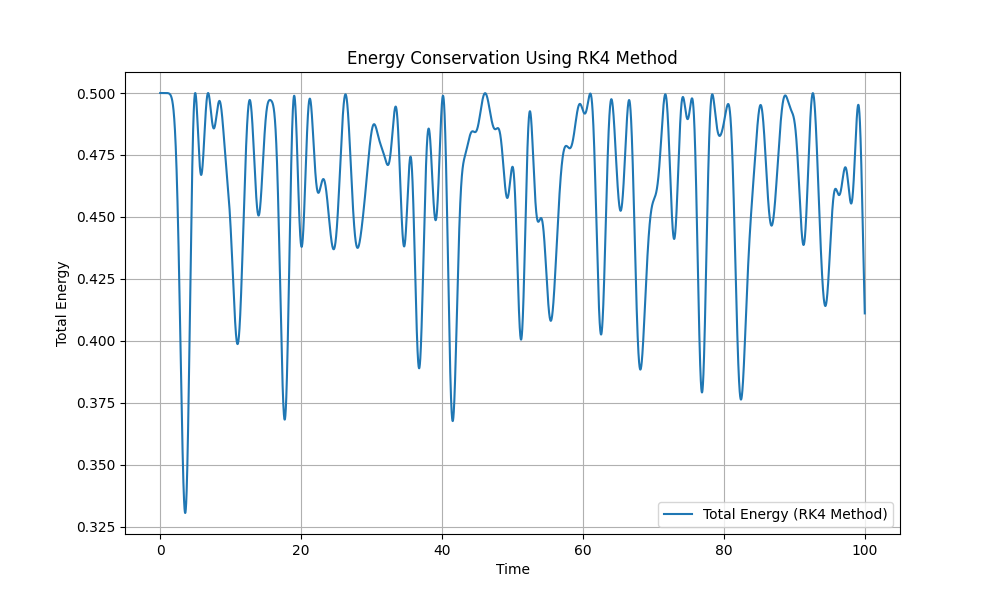
\includegraphics[width=\columnwidth]{4/c2.png}
\end{center}
\lstinputlisting[style = python]{4/b.py}

\answer{c. 结果如下,可以看到跟解析解十分吻合,同样也是没有很好的能量守恒,存在一些较大的波动,整体均值在接近初始能量0.5附近。}
\begin{center}
	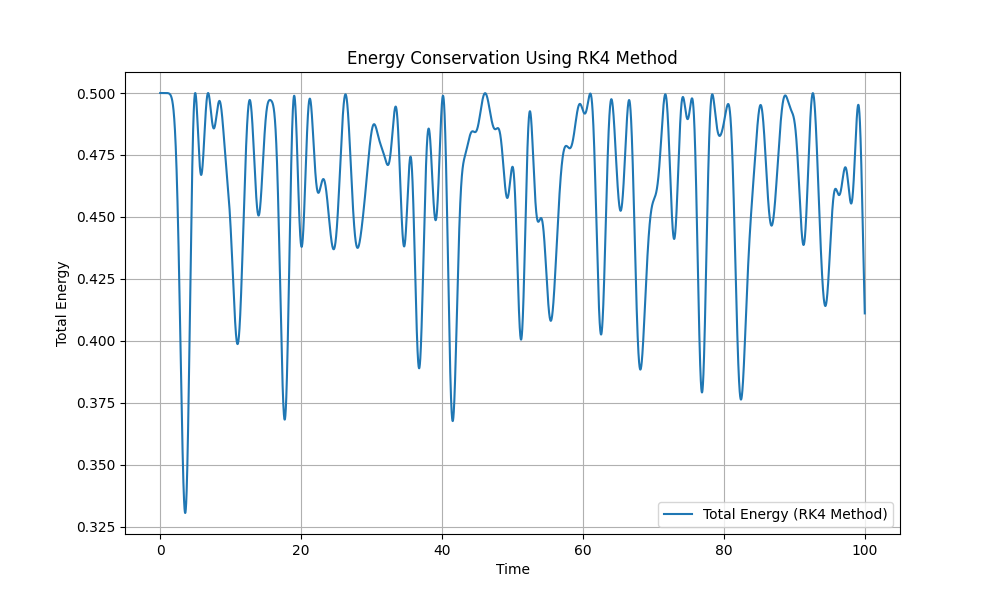
\includegraphics[width=\columnwidth]{4/c1.png}
\end{center}
\lstinputlisting[style = python]{4/a6rk4.py}
\end{question}
\end{document}
